\subsection*{TreeInsert}

Da der Baum T am Anfang leer ist, wird 5 zur Wurzel:

Die while-Schleife wird 0 mal durchlaufen, weil schon zu Beginn x = nil ist. Als Vater von der 5 wird nil eingetragen. Und da der zuletzt besuchte Knoten y noch nil ist, wird 5 als Wurzel von T gesetzt.

\begin{center}
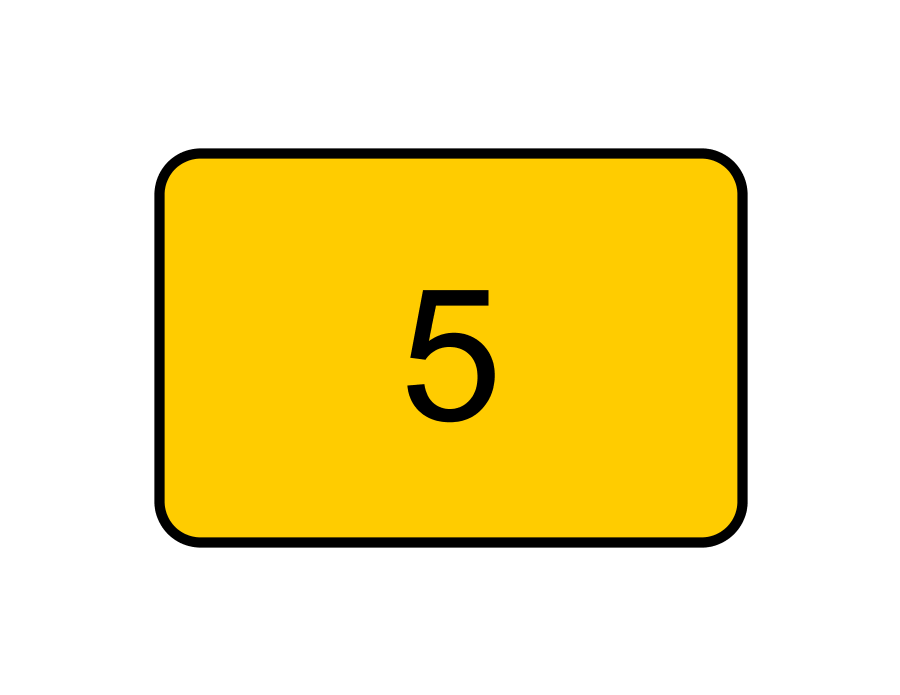
\includegraphics[width=0.1\textwidth]{511-Baeume/1durchgang-5eingefuegt.png}
\end{center}

Der nächste Knoten - die 8 - wird als rechtes Kind von 5 eingefügt, weil 8 nicht kleiner als 5 ist.

\begin{center}
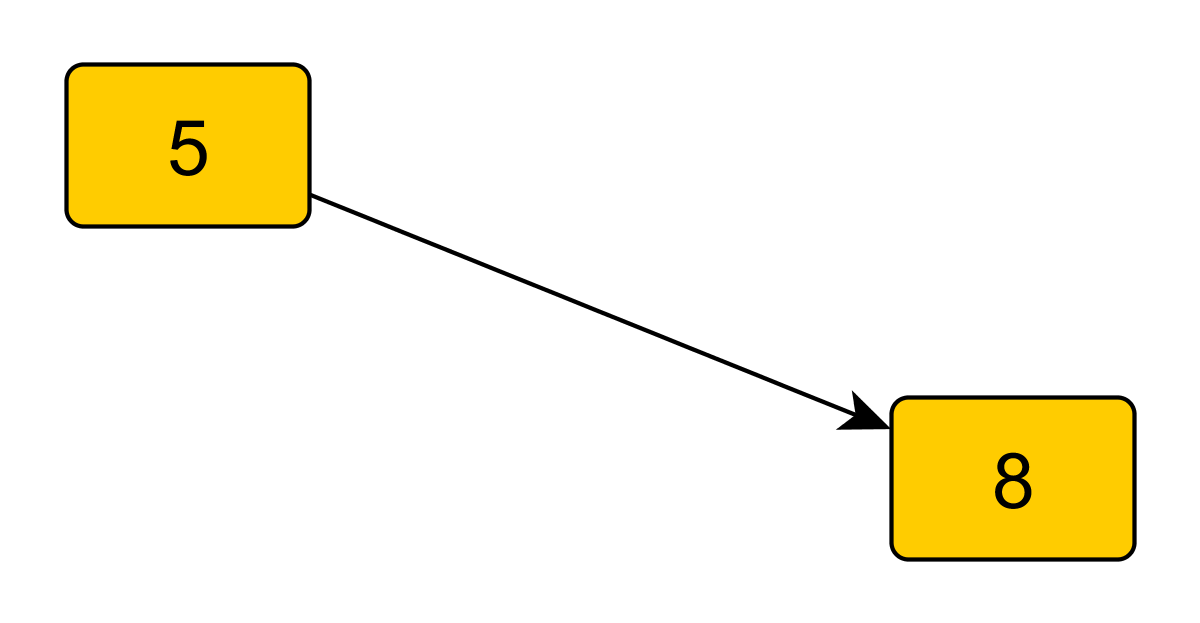
\includegraphics[width=0.3\textwidth]{511-Baeume/2durchgang-8eingefuegt.png}
\end{center}

Die 9 wird als rechtes Kind von 8 eingefügt, weil sie nicht kleiner als 8 ist, nachdem die Operation so von der Wurzel bis zum Blatt gegangen ist, dass der neue Knoten immer links von größeren Vorgängern (hier nicht der Fall) und rechts bei kleineren Vorgängern/Eltern eingefügt würde.

\begin{center}
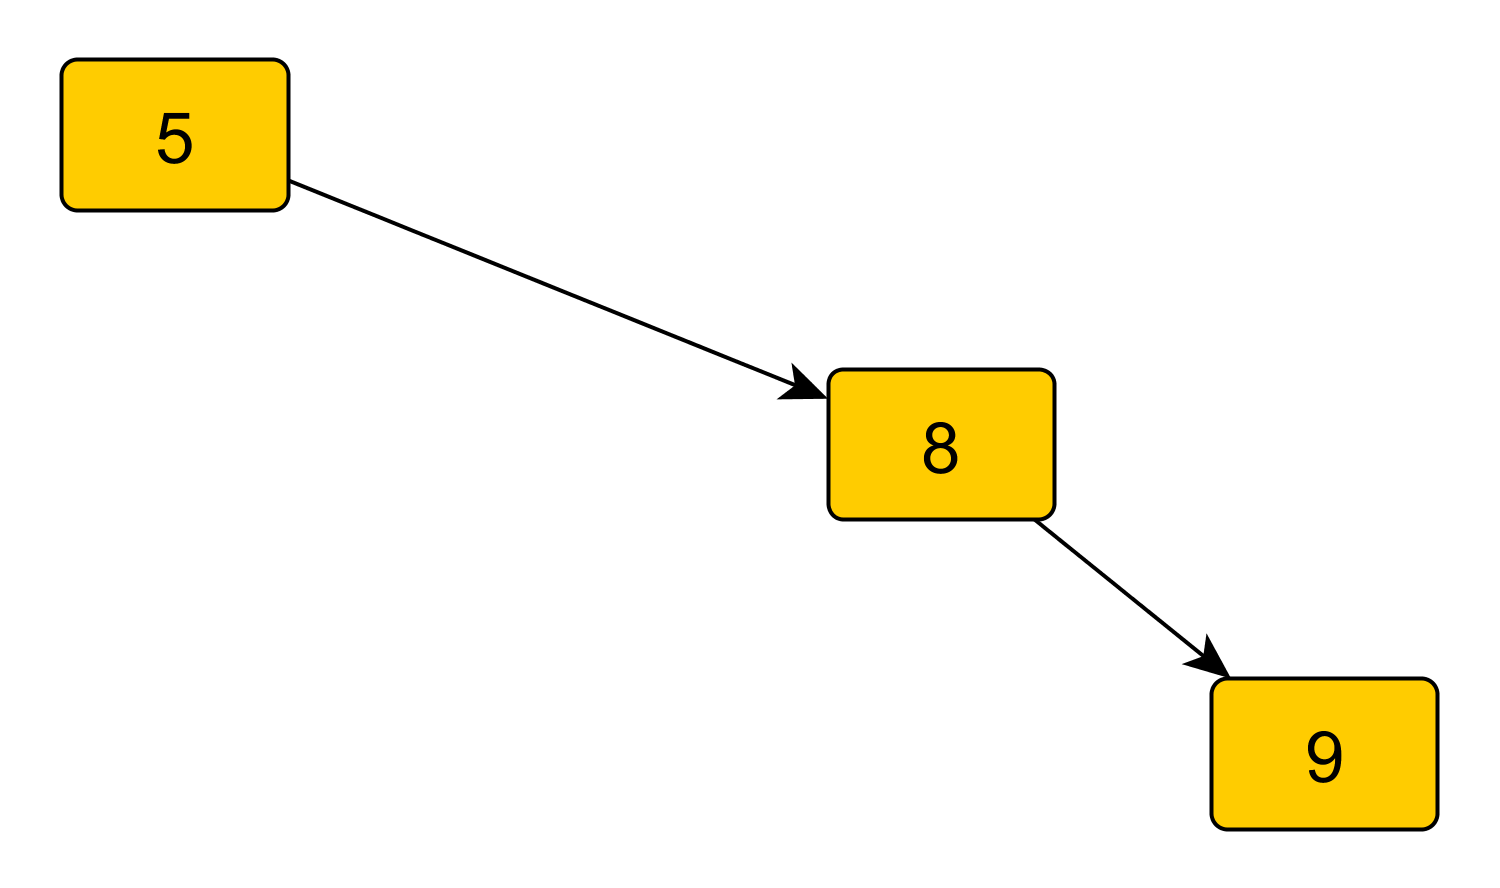
\includegraphics[width=0.45\textwidth]{511-Baeume/3durchgang-9eingefuegt.png}
\end{center}

Zum Einfügen der 6 wird (auch schon in der while Schleife) das linke Kind von 8 gewählt, da 6 kleiner als 8 ist. Da das linke Kind von 8 noch nil war, wird hier die 6 eingefügt.

\begin{center}
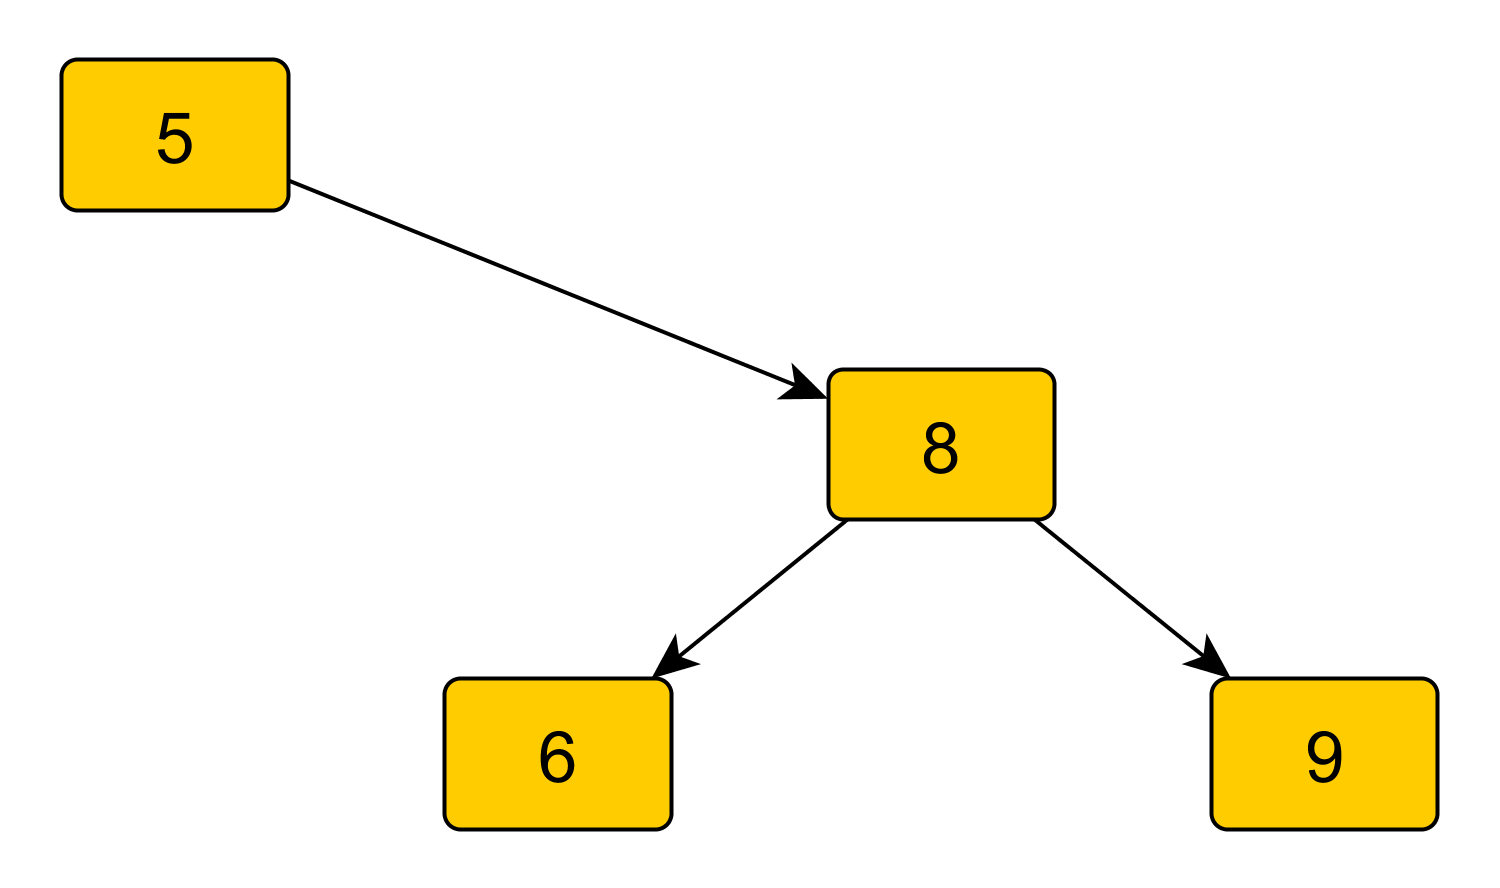
\includegraphics[width=0.45\textwidth]{511-Baeume/4durchgang-6eingefuegt.png}
\end{center}

Die 7 wird als rechtes Kind der 6 hinzugefügt.

\begin{center}
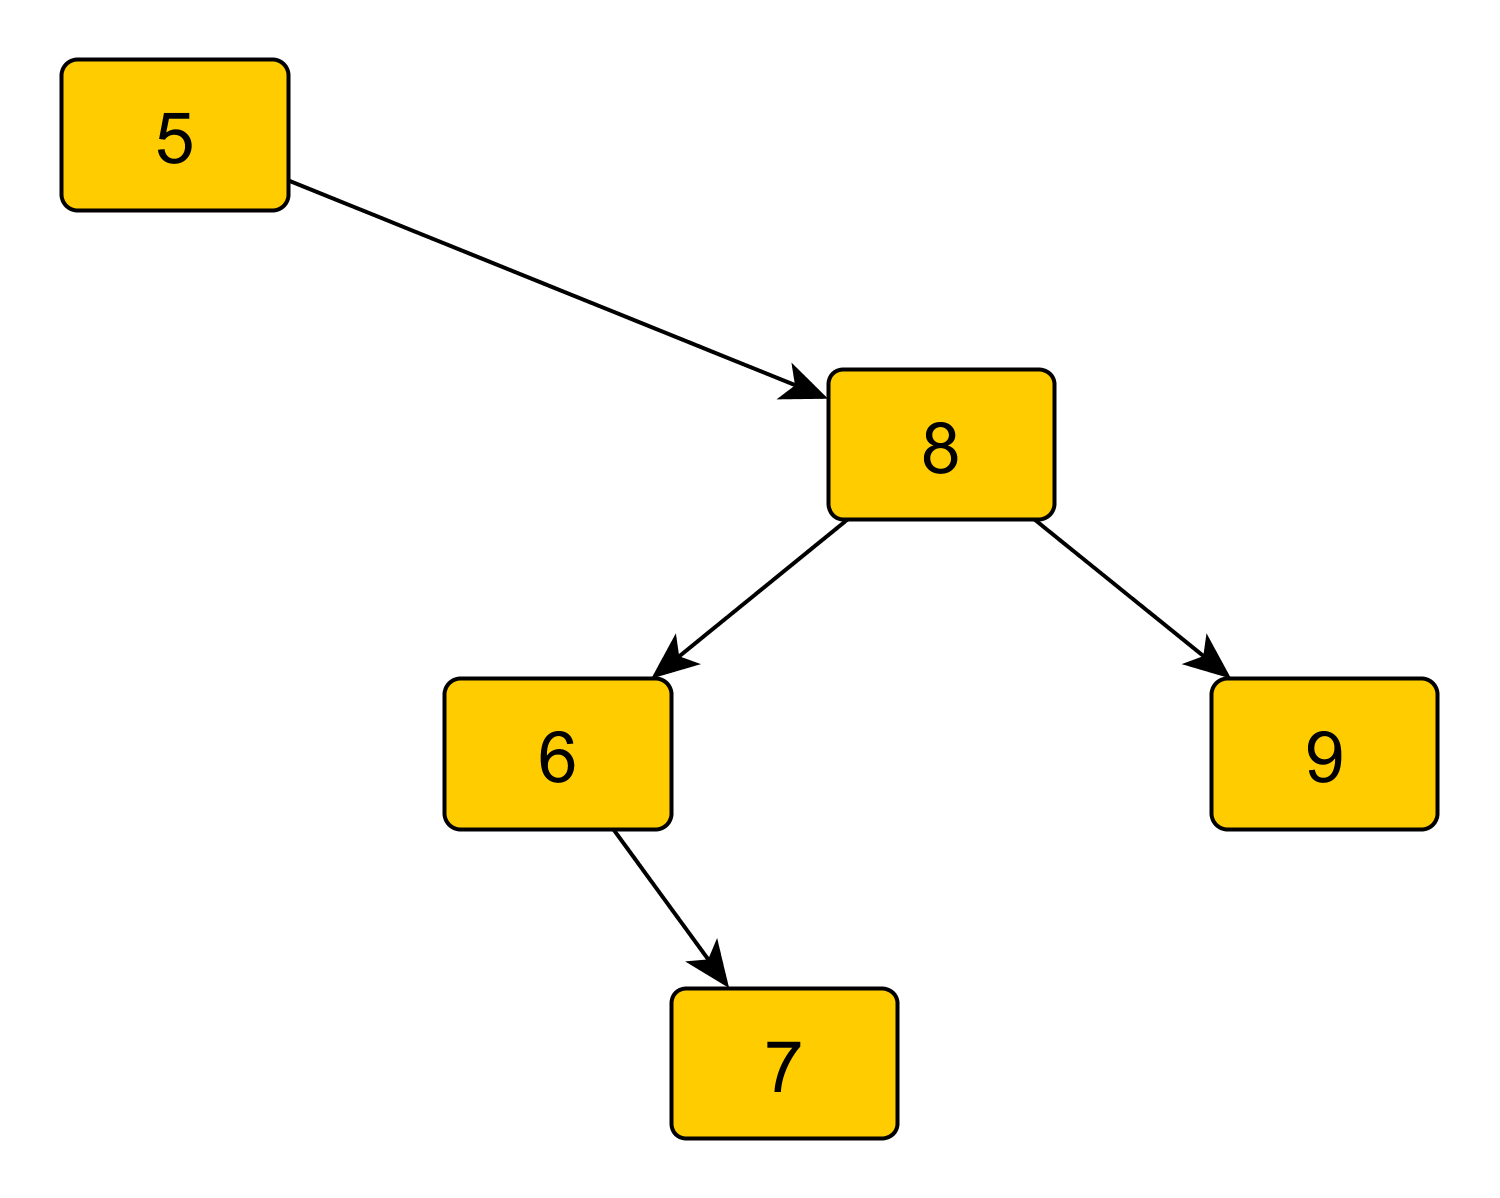
\includegraphics[width=0.45\textwidth]{511-Baeume/5durchgang-7eingefuegt.png}
\end{center}


\subsection*{Löschen}

Da 14 keine Kinder hat, kann der Knoten einfach gelöscht werden.

\begin{center}
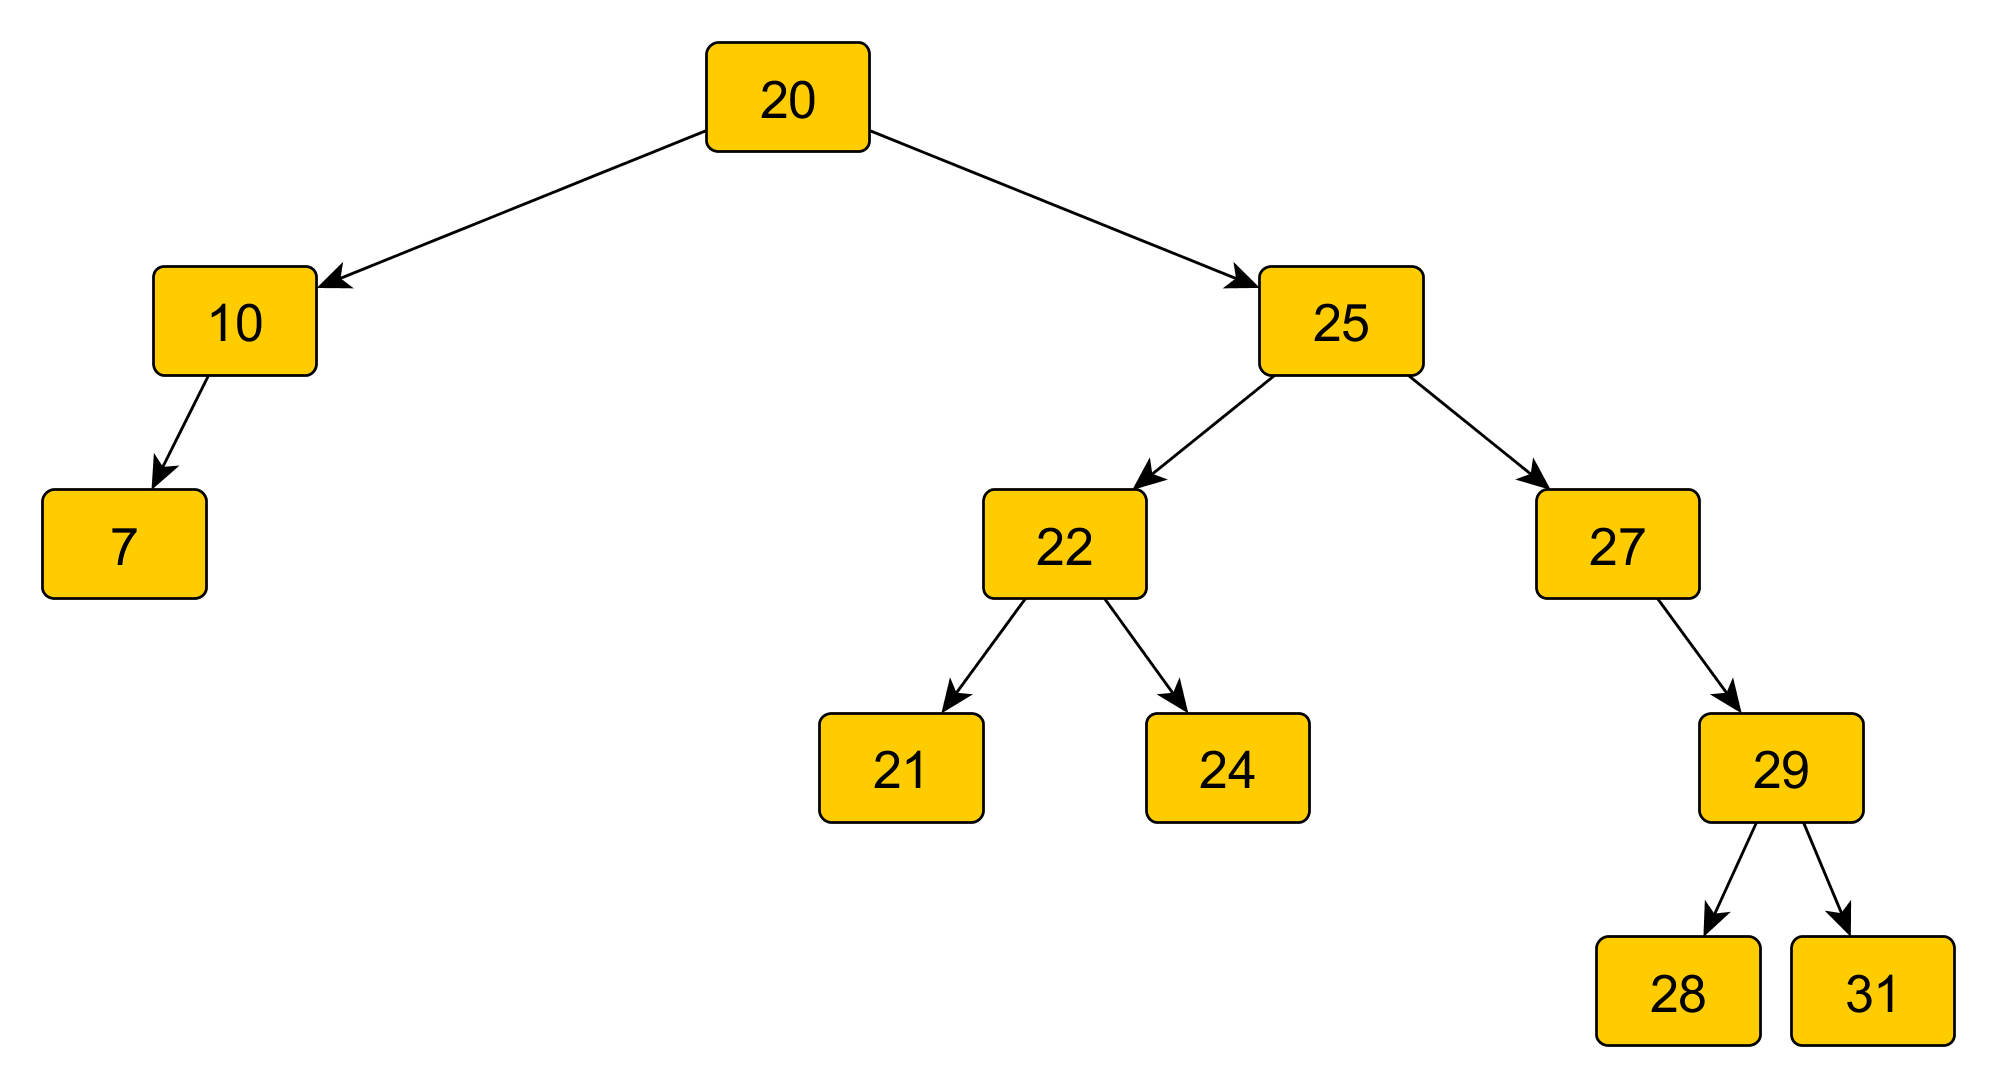
\includegraphics[width=0.8\textwidth]{512-Baume/1durchgang-14loschen.png}
\end{center}

Da 27 nur ein Kind hat, kann der Knoten "ausgeschnitten" werden. Dabei wird die 25 als Vaterknoten der 27 mit der 29 als rechtes Kind verbunden und die 27 kann gelöscht werden.

\begin{center}
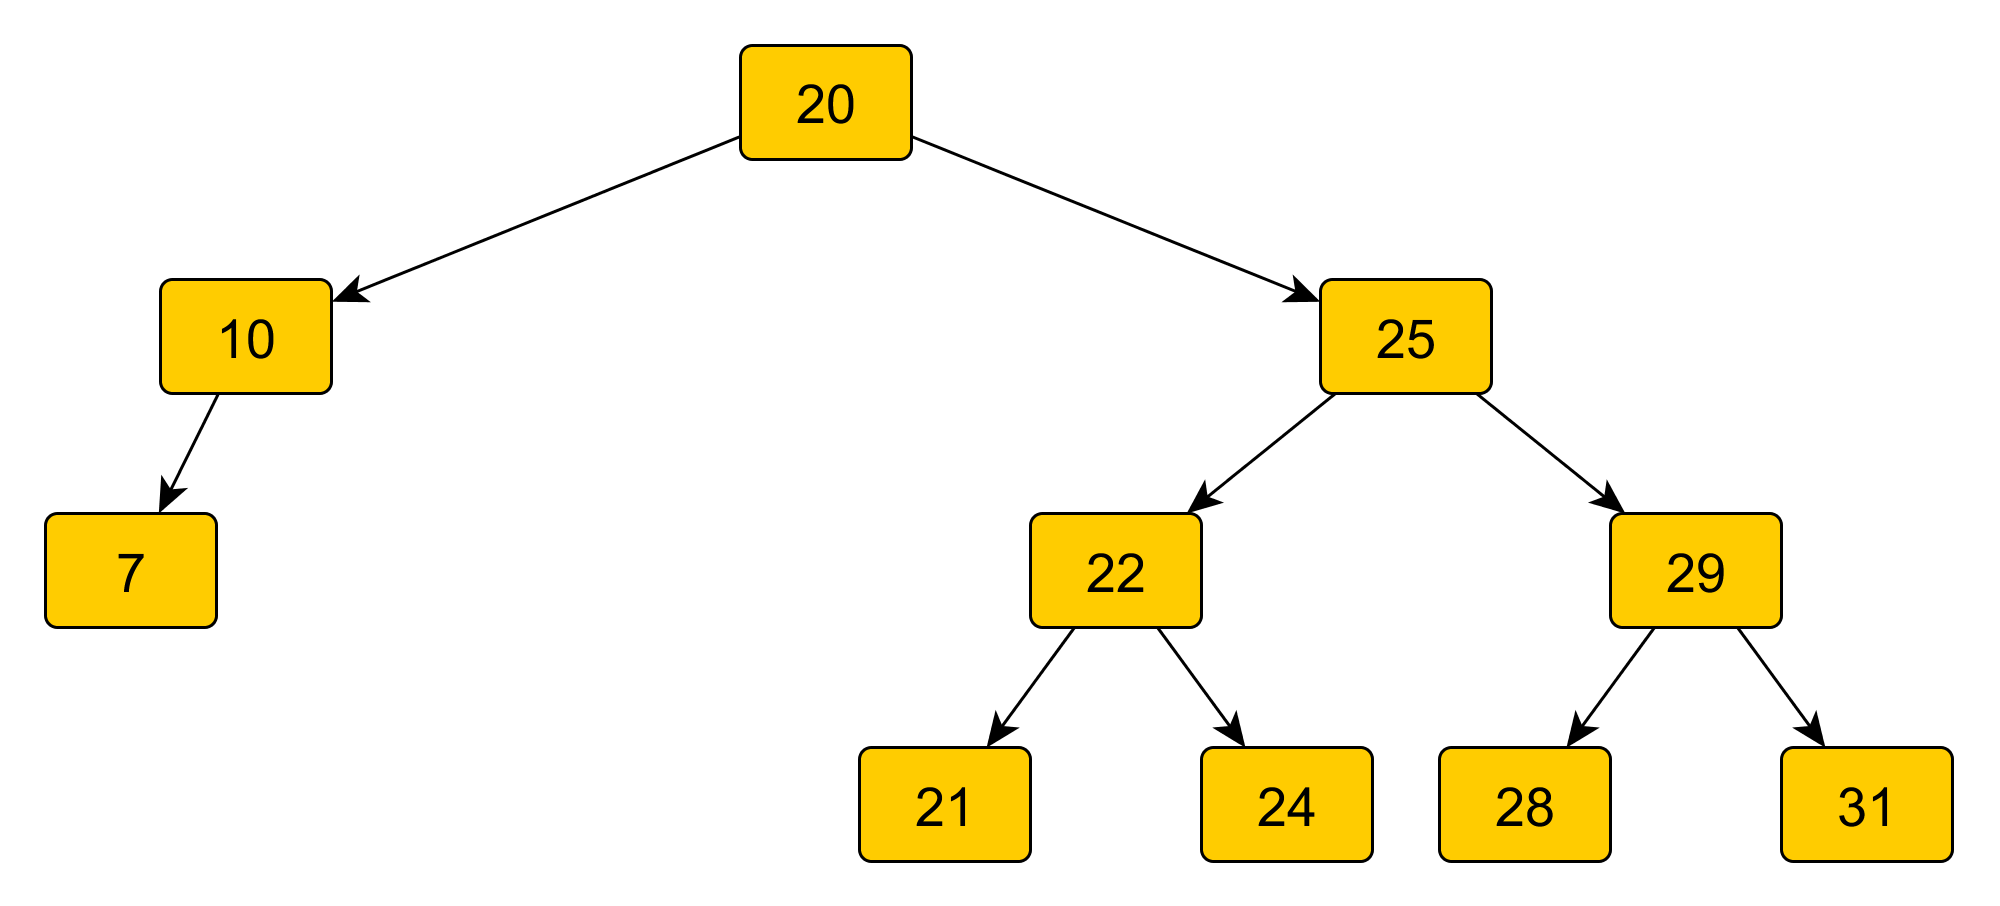
\includegraphics[width=0.8\textwidth]{512-Baume/2durchgang-27loschen.png}
\end{center}

Um die 25 zu löschen muss ihr direkter Nachfolger bestimmt werden. Dazu wird der rechte Teilbaum unter der 25 betrachtet und das Minimum bestimmt. Die 28 wird ausgeschnitten (in diesem Fall einfach gelöscht) und anstelle der 25 eingefügt.

\begin{center}
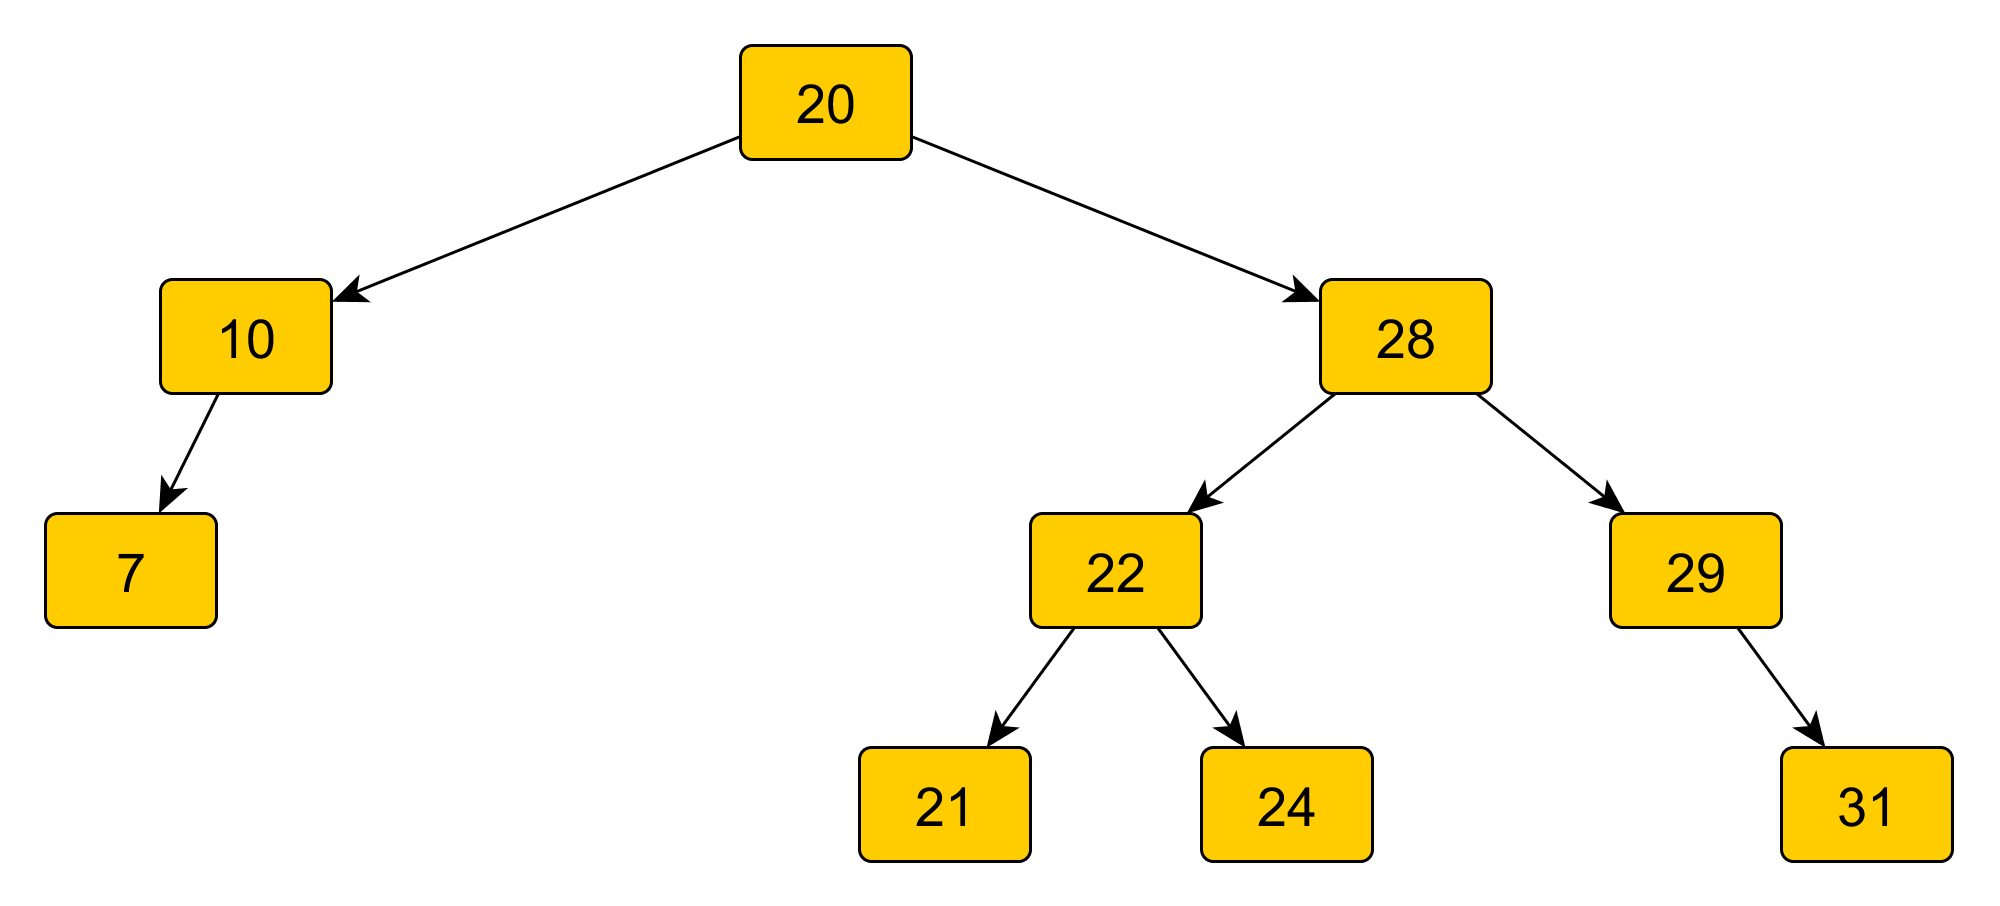
\includegraphics[width=0.8\textwidth]{512-Baume/3durchgang-25loschen.png}
\end{center}